\documentclass[11pt]{article}
\usepackage[margin=1in]{geometry}
\usepackage[T1]{fontenc}
\usepackage{lmodern,amsmath,amssymb,booktabs,graphicx,microtype}
\usepackage[colorlinks=true,allcolors=blue]{hyperref}
\usepackage{placeins}
\title{Stage-Specific Relative Chess Piece Values\\Estimated with One-Step Maximum-Entropy IRL}
\author{Author information pending\\\small Working draft: not submitted}
\date{September 2026}
\begin{document}
\maketitle
\begin{abstract}
We estimate stage-specific relative chess piece values from Stockfish 18 move choices using a one-step maximum-entropy inverse reinforcement learning model. Here, value means a model-conditional action-reward coefficient, not a uniquely identified strategic exchange price. Using 300 self-play games and 18,351 retained positions, we report opening, middlegame, and endgame coefficients normalized to pawn = 1. In the pooled contextual model, knight estimates are 2.64, 1.50, and 0.87; bishop estimates are 4.33, 2.28, and 1.15. We extend the analysis with independent stage fits, alternative context specifications, regularization sensitivity, and alternative stage boundaries. The results expose meaningful specification dependence and limited opening evidence for major-piece coefficients. Game-bootstrap intervals quantify conditional sampling uncertainty. All extensions are exploratory and remain within the same horizon-one IRL family; no claim of a new IRL algorithm or recovery of intrinsic piece prices is made.
\end{abstract}

\section{Introduction}
Relative piece values summarize how a chess decision maker trades material against other features of a position. A single fixed table is convenient, but it conceals potential variation between early development, active middlegame play, and simplified endings. The purpose of this paper is to report and scrutinize IRL-estimated relative piece values at these three stages. Predictive accuracy is retained as a supporting check; the central objects are the coefficients, their uncertainty, and their dependence on modeling choices.

The term ``IRL-estimated value'' has a deliberately restricted meaning here. We infer an immediate action-reward model from demonstrated moves. We neither observe an engine's internal material weights nor recover an exact value of exchanging a piece after optimal future play. In particular, a knight coefficient below the normalized pawn coefficient must not be read as a recommendation to exchange a knight for a pawn. This distinction is essential for interpreting all tables below.

The empirical contributions are a stage-specific value table with game-bootstrap intervals; a comparison between pooled contextual estimation and independently fitted stage models; and sensitivity analyses over context features, ridge penalties, and stage boundaries. These are complementary views of the same data rather than independent replications. They reveal which conclusions depend on pooling, normalization, and available material-choice evidence. The stage analyses were developed after the original experiment and are explicitly exploratory.

\section{Related work}

Learning chess evaluation parameters from played moves has a long history. David et al.\ \cite{david} optimized evaluation functions to imitate grandmaster moves using genetic algorithms, followed by coevolution. Thus, learning from actions without numeric engine labels is not itself a novelty claim here. P\'alsson and Bj\"ornsson\ \cite{palsson} analyzed concepts in a strong chess engine and examined relative material values across game phases. PAWN\ \cite{pawn} predicts position-specific piece values using labels defined by changes in engine evaluation after removing a piece. Our target instead concerns coefficients inferred from selected legal actions; it is not the same estimand as removal-based contribution.

Maximum-entropy IRL provides a probabilistic framework for explaining demonstrations with rewards\ \cite{ziebart}. Our horizon-one specialization is a conditional logit model over legal moves. It should not be confused with trajectory-level inference or a solution to adversarial sequential chess. Reward identification depends on modeling assumptions\ \cite{kim}; regularization and normalization select a numerical representation without proving it to be a unique underlying reward.

\section{One-step maximum-entropy IRL}
\subsection{Immediate action features}
For a pre-move state $s$, let $A(s)$ be all legal moves, and let $s_a$ be the state after move $a$. Fix the perspective to the player moving in $s$. The feature vector $\phi(s)$ consists of own-minus-opponent counts of pawns, knights, bishops, rooks, and queens, a signed centrality sum, an indicator of check delivered to the opponent, and an indicator of delivered mate. Centrality of a piece on zero-indexed file $f$ and rank $r$ is
\[
c(f,r)=\frac{7-|f-3.5|-|r-3.5|}{7}.
\]
Centrality is summed positively for own pieces and negatively for opposing pieces. Define $x(s,a)=\phi(s_a)-\phi(s)\in\mathbb R^8$. No engine evaluation score enters these features or supplies a training label.

\subsection{Context-conditioned coefficients}
Game phase is
\[
p(s)=\min\{1,(n_N+n_B+2n_R+4n_Q)/24\},
\]
where counts include both players. It is one at the standard initial position and zero when no non-pawn material except kings remains. Openness $o(s)$ is the fraction of files that lack at least one color's pawn; it counts semi-open and fully open files together. This is a precisely defined pawn-structure proxy, not a complete measure of positional openness. Both contexts are computed before the candidate move.

Let $x_M$ contain the five material features and $x_U$ the remaining three. The joint reward model is
\begin{align}
r_\theta(s,a)&=w_M(s)^\top x_M(s,a)+u^\top x_U(s,a),\\
w_M(s)&=b+(p(s)-0.5)d+(o(s)-0.5)e.
\end{align}
The global model sets $d=e=0$, while the phase-only and openness-only variants set one of them to zero. These have 8, 13, 13, and 18 parameters, respectively. The joint model is additive in its contexts; it contains no phase--openness interaction. A single shared set of nuisance coefficients $u$ is used in every learned model.

\subsection{Estimation}
At temperature one, the policy is
\[
\pi_\theta(a\mid s)=\frac{\exp r_\theta(s,a)}{\sum_{a'\in A(s)}\exp r_\theta(s,a')}.
\]
We minimize a game-balanced negative log likelihood with ridge regularization:
\[
\mathcal L(\theta)=-\frac1G\sum_{g=1}^G\frac1{n_g}
\sum_{i\in g}\log\pi_\theta(a_i\mid s_i)+\frac\lambda2\|\theta\|_2^2.
\]
For the fixed design matrix this is a convex problem; positive ridge makes the objective strictly convex. We use L-BFGS-B with an analytic gradient. Choose $\lambda\in\{10^{-4},10^{-3},10^{-2}\}$ by validation game-mean NLL without refitting on the test data. The handcrafted baseline uses $(1,3,3.2,5,9,0.6,0.5,15)$ with a positive inverse temperature fitted on training data. A uniform legal-move policy is included.

\subsection{What the coefficients can identify}
For most non-capturing, non-promoting moves, material-count differences are zero. Material coefficients are therefore informed primarily by the alternatives involving captures and promotions. In our training data, 7,201 of 10,795 positions have variation in at least one material feature across legal moves. There are 91 delivered-mate candidate actions. The material features cannot directly encode the long-term value of saving or repositioning a piece. A low coefficient may reflect a missing tactical continuation rather than low strategic importance. Within-state additive reward terms are unidentifiable from softmax probabilities. Temperature is fixed for learned models, but this convention does not resolve other sources of reward ambiguity or feature misspecification. Pawn normalization is a presentation convention, not evidence for a unique universal price.


\section{Data and stage definitions}
\subsection{Self-play data and partitioning}
We use the same fixed dataset throughout: 300 Stockfish 18 self-play games with one thread, a 64 MB hash and 5,000 search nodes per move\ \cite{stockfish}. Games start from standard chess, with eight uniformly sampled legal exploratory plies excluded from fitting. Subsequent moves are chosen by the engine. Every other expert position is sampled, alternating sampled color by game ID. Games stop under a rule-based termination or at 240 plies; the nine length-limited games are marked truncated, not drawn.

Games are assigned 60/20/20 to train, validation, and test using permutation seed 20260927. Forced-choice positions and exact repeated board states are removed, with training taking precedence over validation and test. The state key contains placement, turn, castling, and legal en-passant status; full histories are separately preserved. The retained splits contain 10,795, 3,624, and 3,932 positions. One training game contributes no retained positions, leaving 179, 60, and 60 represented games. This controls exact-state leakage, not all shared motifs or history-dependent effects.

\subsection{Operational stage boundaries}
Let $U=n_N+n_B+2n_R+4n_Q$ count both colors' non-pawn material. An endgame is a state with $U\leq6$, or $p\leq0.25$. This rule takes precedence. An opening is any remaining state through full move 10, equivalently pre-move ply $<20$. The first four full moves are exploratory, so observed opening examples begin at full move 5. All remaining states are middlegames. These operational boundaries do not assert a universally accepted chess taxonomy. The endgame definition can include an early liquidation, while move count alone need not identify an endgame.

\subsection{Stage summaries and uncertainty}
For the pooled contextual model, we first average the pre-move contexts within each game and stage, then average equally across contributing games. Since the raw material model is affine in context, evaluating it at this reference context equals the game-balanced mean raw coefficient. We then divide each mean coefficient by the mean pawn coefficient. This is a ratio of means, not a mean of per-position ratios.

We propagate the existing 100 training-game bootstrap coefficient draws through these fixed reference contexts. The intervals do not include uncertainty in the choice or composition of the reference population, nor hyperparameter-selection uncertainty. Paired stage differences use the same coefficient draw in both stages. All intervals are exploratory pointwise intervals, without simultaneous or multiple-comparison coverage. Ratios are withheld if the estimated pawn coefficient or any bootstrap pawn coefficient is nonpositive or near zero. A positive denominator is a numerical requirement, not a proof of substantive identification.
\begin{table}[htbp]\centering
\small
\caption{Training-stage reference distributions. One game can contribute to multiple stages; stage game counts must not be summed as independent games.}\label{tab:coverage}
\begin{tabular}{lrrrr}
\toprule
Stage & Positions & Games & Mean $p$ & Mean $o$\\\midrule
Opening & 1,071 & 179 & 0.981 & 0.132\\
Middlegame & 5,741 & 179 & 0.667 & 0.546\\
Endgame & 3,983 & 136 & 0.165 & 0.881\\
\bottomrule\end{tabular}\end{table}

\FloatBarrier
\section{Primary stage-specific relative values}
Table~\ref{tab:primary} is the principal result. Figure~\ref{fig:stage} visualizes its uncertainty. In this particular pooled model, minor-piece and rook coefficients decrease relative to the pawn across the three reference populations. This pattern is conditional on the feature representation and the changing positions represented in each stage. Phase and file openness are strongly correlated in training positions ($r=-0.802$), so these comparisons do not isolate causal phase effects.
\begin{table}[htbp]\centering
\small
\caption{Primary result: pooled contextual IRL coefficients normalized to pawn = 1. Brackets are pointwise 95\% game-bootstrap intervals, conditional on fixed stage reference contexts.}\label{tab:primary}
\begin{tabular}{lccc}
\toprule
Piece & Opening & Middlegame & Endgame\\\midrule
Pawn & 1.00 [1.00, 1.00] & 1.00 [1.00, 1.00] & 1.00 [1.00, 1.00]\\
Knight & 2.64 [2.08, 3.62] & 1.50 [1.25, 1.79] & 0.87 [0.59, 1.24]\\
Bishop & 4.33 [3.48, 6.05] & 2.28 [2.07, 2.57] & 1.15 [0.81, 1.41]\\
Rook & 4.36 [3.08, 6.47] & 2.96 [2.58, 3.38] & 2.36 [2.03, 2.78]\\
Queen & 4.58 [3.11, 6.76] & 3.87 [3.27, 4.60] & 3.46 [3.03, 3.88]\\
\bottomrule\end{tabular}\end{table}

\begin{figure}[htbp]\centering
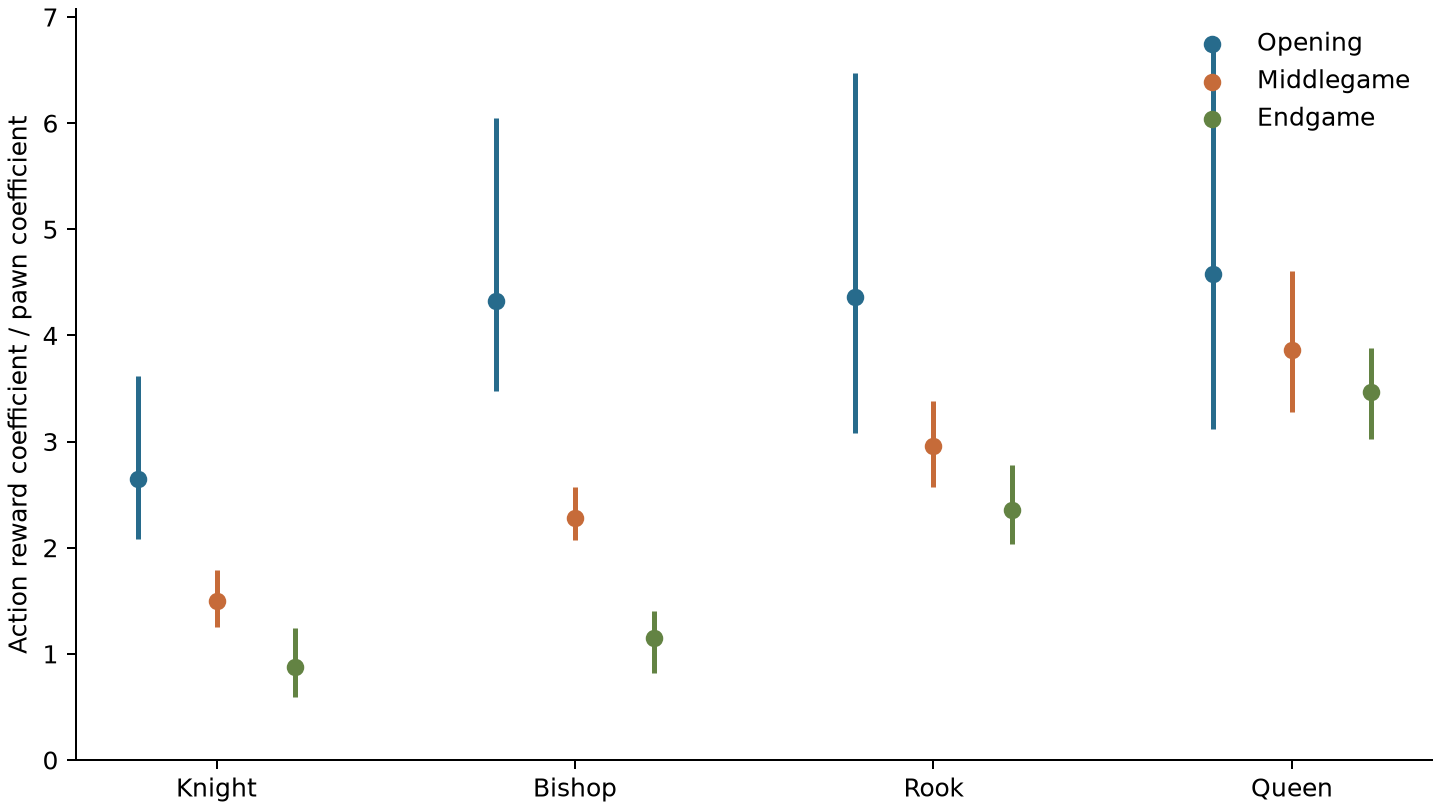
\includegraphics[width=\linewidth]{stage_values.png}
\caption{Pooled contextual IRL relative coefficients by stage. Vertical lines are pointwise 95\% intervals based on 100 game-bootstrap coefficient draws.}\label{fig:stage}
\end{figure}

\subsection{Why raw and normalized values tell different stories}
Table~\ref{tab:raw} reports the unnormalized coefficients. In particular, the pawn coefficient rises from approximately 0.636 in the opening reference population to 1.079 in the endgame population. The queen coefficient also rises, from approximately 2.911 to 3.739, even though its pawn-normalized ratio falls. Thus a decrease in a reported relative value is not evidence that the raw coefficient decreases. Normalization changes the question to value relative to the contemporaneous pawn coefficient.
\begin{table}[htbp]\centering
\small
\caption{Raw action-reward coefficients before pawn normalization. Their common numerical scale is set by temperature one and the selected regularizer.}\label{tab:raw}
\begin{tabular}{lrrr}
\toprule
Piece & Opening & Middlegame & Endgame\\\midrule
Pawn & 0.636 & 0.859 & 1.079\\
Knight & 1.681 & 1.289 & 0.943\\
Bishop & 2.751 & 1.955 & 1.241\\
Rook & 2.773 & 2.541 & 2.542\\
Queen & 2.911 & 3.322 & 3.739\\
\bottomrule\end{tabular}\end{table}
\begin{table}[htbp]\centering
\small
\caption{Endgame minus opening differences in normalized coefficients of the pooled model, using paired bootstrap draws. Intervals are exploratory, pointwise, and not multiplicity-adjusted.}\label{tab:contrast}
\begin{tabular}{lrr}
\toprule
Piece & Difference & 95\% interval\\\midrule
Knight & -1.77 & [-2.73, -0.93]\\
Bishop & -3.18 & [-5.09, -2.09]\\
Rook & -2.00 & [-4.09, -0.54]\\
Queen & -1.11 & [-3.20, 0.29]\\
\bottomrule\end{tabular}\end{table}

For knight, bishop, and rook, the displayed paired opening-to-endgame difference intervals exclude zero in the pooled model. The queen difference interval includes zero. These are conditional, exploratory comparisons; they do not justify a general law that each piece loses strategic value as the game progresses.

\FloatBarrier
\section{Different IRL model specifications}
\subsection{Global, phase-only, openness-only, and joint models}
The global, phase-only, openness-only, and joint specifications have 8, 13, 13, and 18 parameters. All share the same immediate features, temperature convention, game-balanced objective, and validation procedure. Table~\ref{tab:family} evaluates them at the same stage reference distributions. By construction the global model cannot express stage variation. Phase-only and openness-only models attribute differences to distinct correlated covariates. Their disagreement is therefore informative about specification dependence rather than evidence that one covariate is a causal explanation.
\begin{table}[htbp]\centering
\small
\caption{Alternative specifications of the same one-step maximum-entropy IRL family, evaluated at identical stage contexts. Pawn = 1. These are not four different IRL algorithms.}\label{tab:family}
\begin{tabular}{llrrrr}
\toprule
Model & Stage & N & B & R & Q\\\midrule
Global & Opening & 1.54 & 2.22 & 2.85 & 4.00\\
Global & Middlegame & 1.54 & 2.22 & 2.85 & 4.00\\
Global & Endgame & 1.54 & 2.22 & 2.85 & 4.00\\
\addlinespace
Phase & Opening & 2.13 & 3.31 & 3.38 & 4.38\\
Phase & Middlegame & 1.53 & 2.29 & 2.89 & 3.95\\
Phase & Endgame & 0.91 & 1.22 & 2.39 & 3.51\\
\addlinespace
Openness & Opening & 2.60 & 4.26 & 4.43 & 4.57\\
Openness & Middlegame & 1.50 & 2.26 & 2.97 & 3.86\\
Openness & Endgame & 0.94 & 1.27 & 2.24 & 3.50\\
\addlinespace
Joint & Opening & 2.64 & 4.33 & 4.36 & 4.58\\
Joint & Middlegame & 1.50 & 2.28 & 2.96 & 3.87\\
Joint & Endgame & 0.87 & 1.15 & 2.36 & 3.46\\
\addlinespace
\bottomrule\end{tabular}\end{table}

These are variants of one maximum-entropy conditional-choice estimator. We do not label them as separate algorithms such as Bayesian IRL, maximum-margin IRL, or adversarial IRL. No experiments with those algorithms were run. The comparison addresses how much the relative coefficients change when context is represented differently.

\subsection{Independent estimation within each stage}
As a complementary analysis, we fit a separate eight-coefficient model to each stage's training positions. We choose ridge strength from the same three-value grid using that stage's validation positions, and perform 100 training-game cluster-bootstrap refits per stage at the selected penalty. Each stage has its own nuisance coefficients for centrality, check, and mate. Unlike the pooled summary, these estimates do not borrow coefficient constraints from other stages.
\begin{table}[htbp]\centering
\small
\caption{Independently fitted stage models: each stage has its own eight coefficients and validation-selected ridge. Brackets are 95\% intervals from 100 bootstrap refits per stage.}\label{tab:independent}
\begin{tabular}{lccc}
\toprule
Piece & Opening & Middlegame & Endgame\\\midrule
Pawn & 1.00 [1.00, 1.00] & 1.00 [1.00, 1.00] & 1.00 [1.00, 1.00]\\
Knight & 1.22 [0.29, 2.22] & 1.92 [1.64, 2.42] & 0.70 [0.13, 1.22]\\
Bishop & 3.46 [2.58, 5.47] & 2.83 [2.45, 3.47] & 0.76 [0.18, 1.33]\\
Rook & 6.81 [5.21, 11.31] & 3.41 [2.96, 4.12] & 2.00 [1.53, 2.56]\\
Queen & 4.50 [1.64, 6.80] & 4.31 [3.55, 5.19] & 3.65 [3.12, 4.50]\\
\bottomrule\end{tabular}\end{table}

The independently fitted opening estimates differ substantially from the pooled opening summary. This is a change in estimator and information sharing, not an independent replication of the same quantity. An independent model approximates the conditional choices within a stage with one fixed vector, while the pooled model uses a continuous context-dependent function learned across stages. Their different normalization denominators and nuisance coefficients can further change the ratios. Cross-stage comparisons of the independent fits should therefore be treated cautiously.

\subsection{How much direct material-choice evidence is available?}
Table~\ref{tab:support} counts positions in which at least one legal action differs in the corresponding material feature. For example, an opening position with no way to change either side's rook count does not directly distinguish rook reward weights through the material component. The opening sample contains only 13 rook-informative and 10 queen-informative positions. A wide interval or large independent opening estimate should be interpreted in light of this scarcity. The counts do not imply that all informative positions are independent observations or that the expert selected a capture.
\begin{table}[htbp]\centering
\small
\caption{Number of training positions whose candidate moves differ in each material feature. These are opportunities to constrain that coefficient, not counts of expert captures.}\label{tab:support}
\begin{tabular}{lrrrrr}
\toprule
Stage & Pawn & Knight & Bishop & Rook & Queen\\\midrule
Opening & 806 & 189 & 46 & 13 & 10\\
Middlegame & 4250 & 1542 & 986 & 653 & 272\\
Endgame & 1214 & 327 & 300 & 251 & 170\\
\bottomrule\end{tabular}\end{table}

\FloatBarrier
\section{Sensitivity analyses}
\subsection{Regularization strength}
Table~\ref{tab:ridge} uses the weights already fitted at all three ridge settings in the original validation grid. The reference contexts are held fixed. This separates numerical regularization sensitivity from changes in stage composition. Larger ridge penalties shrink raw coefficients, but ratios need not shrink uniformly because both numerator and pawn denominator change. We report every grid setting, including those not selected by validation, rather than selecting the most intuitive value table.
\begin{table}[htbp]\centering
\small
\caption{Ridge sensitivity of the pooled joint model at the same reference contexts. No test results were used to select these settings; all three original grid values are displayed.}\label{tab:ridge}
\begin{tabular}{rlrrrr}
\toprule
$\lambda$ & Stage & N & B & R & Q\\\midrule
0.0001 & Opening & 2.64 & 4.33 & 4.36 & 4.58\\
0.0001 & Middlegame & 1.50 & 2.28 & 2.96 & 3.87\\
0.0001 & Endgame & 0.87 & 1.15 & 2.36 & 3.46\\
\addlinespace
0.001 & Opening & 2.52 & 3.97 & 3.89 & 4.38\\
0.001 & Middlegame & 1.51 & 2.31 & 2.90 & 3.76\\
0.001 & Endgame & 0.89 & 1.25 & 2.33 & 3.39\\
\addlinespace
0.01 & Opening & 1.94 & 2.85 & 2.66 & 2.70\\
0.01 & Middlegame & 1.45 & 2.17 & 2.43 & 2.62\\
0.01 & Endgame & 1.02 & 1.58 & 2.24 & 2.55\\
\addlinespace
\bottomrule\end{tabular}\end{table}

The validation-selected penalties lie on the lower boundary of the tested grid. The study does not establish optimality over penalties outside that grid. The displayed sensitivity is descriptive and does not supply confidence intervals for choosing between regularizers.

\subsection{Stage-boundary sensitivity}
We vary the last opening full move from 10 to 8 or 12, and the endgame material threshold from 6 to 4 or 8, changing one definition at a time. Table~\ref{tab:boundary} shows all settings. The fitted joint model is unchanged: these results measure changes in the reference population, not new IRL training runs. Consequently, similar numbers across nearby cutoffs demonstrate local stability of this summary procedure, not robustness to an entirely different model or dataset.
\begin{table}[htbp]\centering
\small
\caption{Sensitivity to the stage definition. Settings are opening last full move / endgame material-unit threshold. The model is frozen; only the reference populations change. Pawn = 1.}\label{tab:boundary}
\begin{tabular}{llrrrr}
\toprule
Definition & Stage & N & B & R & Q\\\midrule
10 / 6 & Opening & 2.64 & 4.33 & 4.36 & 4.58\\
10 / 6 & Middlegame & 1.50 & 2.28 & 2.96 & 3.87\\
10 / 6 & Endgame & 0.87 & 1.15 & 2.36 & 3.46\\
\addlinespace
8 / 6 & Opening & 2.75 & 4.53 & 4.52 & 4.64\\
8 / 6 & Middlegame & 1.55 & 2.36 & 3.01 & 3.90\\
8 / 6 & Endgame & 0.87 & 1.15 & 2.36 & 3.46\\
\addlinespace
12 / 6 & Opening & 2.54 & 4.14 & 4.22 & 4.51\\
12 / 6 & Middlegame & 1.45 & 2.19 & 2.91 & 3.84\\
12 / 6 & Endgame & 0.87 & 1.15 & 2.36 & 3.46\\
\addlinespace
10 / 4 & Opening & 2.64 & 4.33 & 4.36 & 4.58\\
10 / 4 & Middlegame & 1.39 & 2.07 & 2.84 & 3.80\\
10 / 4 & Endgame & 0.83 & 1.07 & 2.31 & 3.44\\
\addlinespace
10 / 8 & Opening & 2.64 & 4.33 & 4.36 & 4.58\\
10 / 8 & Middlegame & 1.61 & 2.47 & 3.07 & 3.94\\
10 / 8 & Endgame & 0.90 & 1.20 & 2.37 & 3.48\\
\addlinespace
\bottomrule\end{tabular}\end{table}

\FloatBarrier
\section{Piece-wise interpretation}
\paragraph{Pawn.} Every normalized table sets the pawn to one by division, not by constraining its learned coefficient to be constant. The raw estimates expose its changing role in the normalization. They also show why ratios alone cannot establish whether another piece's raw contribution rose or fell.
\paragraph{Knight.} The pooled stage summaries decline strongly, but the independent opening estimate is lower than the pooled opening estimate. This discrepancy cautions against interpreting a single early-game number as a stable exchange price. In endgames, a ratio below one is a property of the fitted immediate-choice model; it does not establish that a knight is strategically inferior to a pawn.
\paragraph{Bishop.} The pooled opening ratio is relatively large and has a wide interval. It decreases in later reference populations. The context specifications and independent-stage table expose how much of this pattern depends on cross-stage pooling and on the file-openness proxy. No causal claim about opening a file or preserving a bishop pair is tested.
\paragraph{Rook.} The difference between pooled and independent opening fits is especially relevant because only a small number of opening positions can constrain rook-count preferences. Rook estimates should be reported with their uncertainty and support counts rather than rounded into a new fixed chess rule.
\paragraph{Queen.} Its raw coefficient and normalized ratio move in opposite directions across the pooled opening and endgame references. The opening-to-endgame normalized difference interval includes zero. The results therefore do not establish a consistent queen-value decrease. Opening queen evidence is particularly sparse.

\section{Limitations and conclusion}
The paper estimates model-conditional, stage-specific relative piece values within a horizon-one IRL family. Immediate feature differences cannot represent a future recapture, a mating combination several plies away, or the long-term benefit of retaining a piece. Quiet non-promoting moves usually have zero material difference. Missing continuations and omitted positional features can be absorbed into coefficients. These limitations explain why the tables must not be treated as universally valid strategic prices, although they do not quantify which omission causes each observed discrepancy.

The results come from one engine version, one node budget, random early exploration, one main game collection, and one train/validation/test split. Bootstrap intervals measure conditional sampling variation rather than generalization across engines or stronger search. Stage boundaries are operational, and phases differ in both material and pawn structure. The pooled and independent estimators have different sharing assumptions. All follow-up analyses were motivated after observing the original run and should be read as exploratory. There is no claim of a new IRL algorithm, a new discovery that piece values are contextual, or improved match strength.

The principal output is a transparent stage-specific value table together with comparisons that expose its dependence on estimation choices. Reporting pooled and independent fits, raw and normalized coefficients, and sensitivity to penalties and boundaries is more informative than presenting one numerical table as definitive. The data support further investigation with reply-aware features and independent collections, while the current results form a reproducible restricted baseline.

\section*{Data, code, and tool use}
The accompanying archive includes the full 300-game self-play data, original and extended fitting code, selected models, bootstrap coefficients, stage definitions, and machine-readable tables. The original protocol remains unchanged; an extension note records that these analyses were added later. OpenAI Codex assisted in research design, implementation, analysis, and manuscript drafting. Numerical results are computed by the supplied programs. Author identity and final author review remain required before submission; the work has not been submitted to arXiv.

\appendix
\section{Supporting predictive checks}
Behavioral prediction is not the main result, but it checks whether estimated rewards bear a measurable relationship to held-out move choices. Table~\ref{tab:performance} retains the original model comparison. The joint minus global game-mean NLL difference is -0.0057 nats, with a paired 95\% game-bootstrap interval [-0.0095, -0.0017]. The effect is small. A lower prediction loss does not establish that a coefficient is an intrinsic material value.
\begin{table}[htbp]\centering
\small
\caption{Supporting held-out behavioral prediction, retained as a validity diagnostic rather than the main research outcome.}\label{tab:performance}
\begin{tabular}{lrr}
\toprule
Model & Game-mean NLL & Top-1 (\%)\\\midrule
Uniform & 3.1008 & 6.70\\
Handcrafted & 2.9337 & 16.79\\
Global & 2.9044 & 16.70\\
Phase & 2.9010 & 16.90\\
Openness & 2.8993 & 16.90\\
Joint & 2.8987 & 16.96\\
\bottomrule\end{tabular}\end{table}
\begin{table}[htbp]\centering
\small
\caption{Exploratory stage-level prediction diagnostics. Independent fits are evaluated only on their corresponding held-out stage. No model is selected using this table.}\label{tab:stageperf}
\begin{tabular}{lrrrr}
\toprule
Stage & Test games & Global NLL & Joint NLL & Independent NLL\\\midrule
Opening & 60 & 3.2233 & 3.2040 & 3.2225\\
Middlegame & 60 & 3.0621 & 3.0568 & 3.0622\\
Endgame & 53 & 2.4270 & 2.4257 & 2.4295\\
\bottomrule\end{tabular}\end{table}

\FloatBarrier
\section{Reproducibility and numerical checks}
The original analytic-gradient check had maximum absolute error $3.75\times10^{-11}$, and a synthetic conditional-choice recovery test had coefficient RMSE 0.0386. Perspective, promotion, legal candidate enumeration, board restoration, and game weighting were tested. Collected histories were replayed to verify stored states and moves. The extension additionally verifies that stage-subset target rows equal the corresponding original chosen-action feature rows and that subset game weights sum to one.

Original bootstrap coefficients are used only for pooled stage summaries. Independent-stage intervals come from 300 additional refits, 100 per stage, with stage-specific penalties fixed after validation. Stage subsetting does not move any game across the original train/validation/test partition. Neither context cutoffs nor the displayed sensitivity settings are selected using test performance. Package versions, full configurations, code hashes, and engine hashes accompany the numerical results. No fabricated value table or unexecuted algorithm is presented as an experiment.
\FloatBarrier
\begin{thebibliography}{9}\small
\bibitem{david} E. David, H. J. van den Herik, M. Koppel, and N. S. Netanyahu. Simulating Human Grandmasters: Evolution and Coevolution of Evaluation Functions. In \emph{GECCO}, pp. 1483--1489, 2009. \href{https://arxiv.org/abs/1711.06840}{arXiv:1711.06840}.
\bibitem{palsson} A. P\'alsson and Y. Bj\"ornsson. Unveiling Concepts Learned by a World-Class Chess-Playing Agent. In \emph{IJCAI}, 2023. \href{https://www.ijcai.org/proceedings/2023/541}{Proceedings}.
\bibitem{pawn} E. Tang, H. Davulcu, J. Zou, and Z. Zhang. PAWN: Piece Value Analysis with Neural Networks. \href{https://arxiv.org/abs/2604.15585}{arXiv:2604.15585}, 2026.
\bibitem{ziebart} B. D. Ziebart, A. Maas, J. A. Bagnell, and A. K. Dey. Maximum Entropy Inverse Reinforcement Learning. In \emph{AAAI}, pp. 1433--1438, 2008. \href{https://www.cs.cmu.edu/~bziebart/publications/maximum-entropy-inverse-reinforcement-learning.html}{Paper}.
\bibitem{kim} K. Kim, S. Garg, K. Shiragur, and S. Ermon. Reward Identification in Inverse Reinforcement Learning. In \emph{ICML}, PMLR 139:5496--5505, 2021. \href{https://proceedings.mlr.press/v139/kim21c.html}{Paper}.
\bibitem{stockfish} Stockfish developers. Stockfish 18, 2026. \href{https://github.com/official-stockfish/Stockfish/releases/tag/sf_18}{Official release}.
\end{thebibliography}
\end{document}
